\chapter{Analisi delle pareti esterne}
Sono stati scelti vari materiali e che verranno riportati nei paragrafi successivi con un'apposita descrizione.  
Come si vedrà in seguito, per ogni categoria sono stati valutati aspetti diversi, in quanto in alcuni casi diventavano del tutto trascurabili e alla pari tra i contendenti.

Come prima cosa è stata fatta un'analisi del valore per tutti i materiali in modo da riuscire ad avere un termine di confronto tra i materiali con diversi costi ma con proprietà molto diverse. 
Nell'analisi del valore riportata a pagina \pageref{fig:AnalisiValore} sono stati utilizzati i criteri che vengono riportati nella norma \textsc{UNI 829-2:1983}.
Per ogni criterio è stato assegnato un punteggio da 1 a 5  e utilizzando le caratteristiche riportate dalle aziende produttrici o dall'esperienza. 
Infine si è trovato il totale sommandoli. 
Come risulterà dalle analisi che verranno ora riportate, i maggiori punteggi ottenuti da ciascun materiale, corrispondono anche ai maggiori costi di essi.
Per alcuni risulterà talmente maggiore da non consentire nemmeno di poter fare un'analisi più approfondita.

Si elencano ora i diversi criteri che sono stati tenuti in conto.
Per tutte le categorie è stato calcolato il costo del materiale, preso da prezzario o da analisi prezzi.
A seconda dell'incidenza sono state prese come termine di paragone tempo di posa, manutenzione e spessore risparmiato.
Per quanto riguarda il tempo di posa i dati sono stati ottenuti dal tempario \textcite{grosso2007tempario} e convertiti in euro utilizzando il prezzo unitario dell'operaio (comune o specializzato). 
Nel caso del rivestimento è stato necessario elaborare un piano di manutenzione, come si vedrà in seguito. 
In questo caso è stato valutato come molto incidente i costi che si avranno successivamente alla costruzione dell'edificio.
Lo spessore minore di alcuni strati è stato utilizzato per calcolare la superficie libera risparmiata rispetto alla soluzione zero. 
Si è supposto poi di poter recuperare dei soldi da tale superficie vendendola o affittandola.
Sono stati presi i valori analizzando i prezzi di mercato forniti dall'Agenzia delle Entrate a Trento e ottenendo così un  prezzo di vendita di \SI{3000}{\teuro / \square\metre} e di di affitto di \SI{10.41}{\teuro /\square\metre mese }.


\begin{figure}[p]
    \centering 
    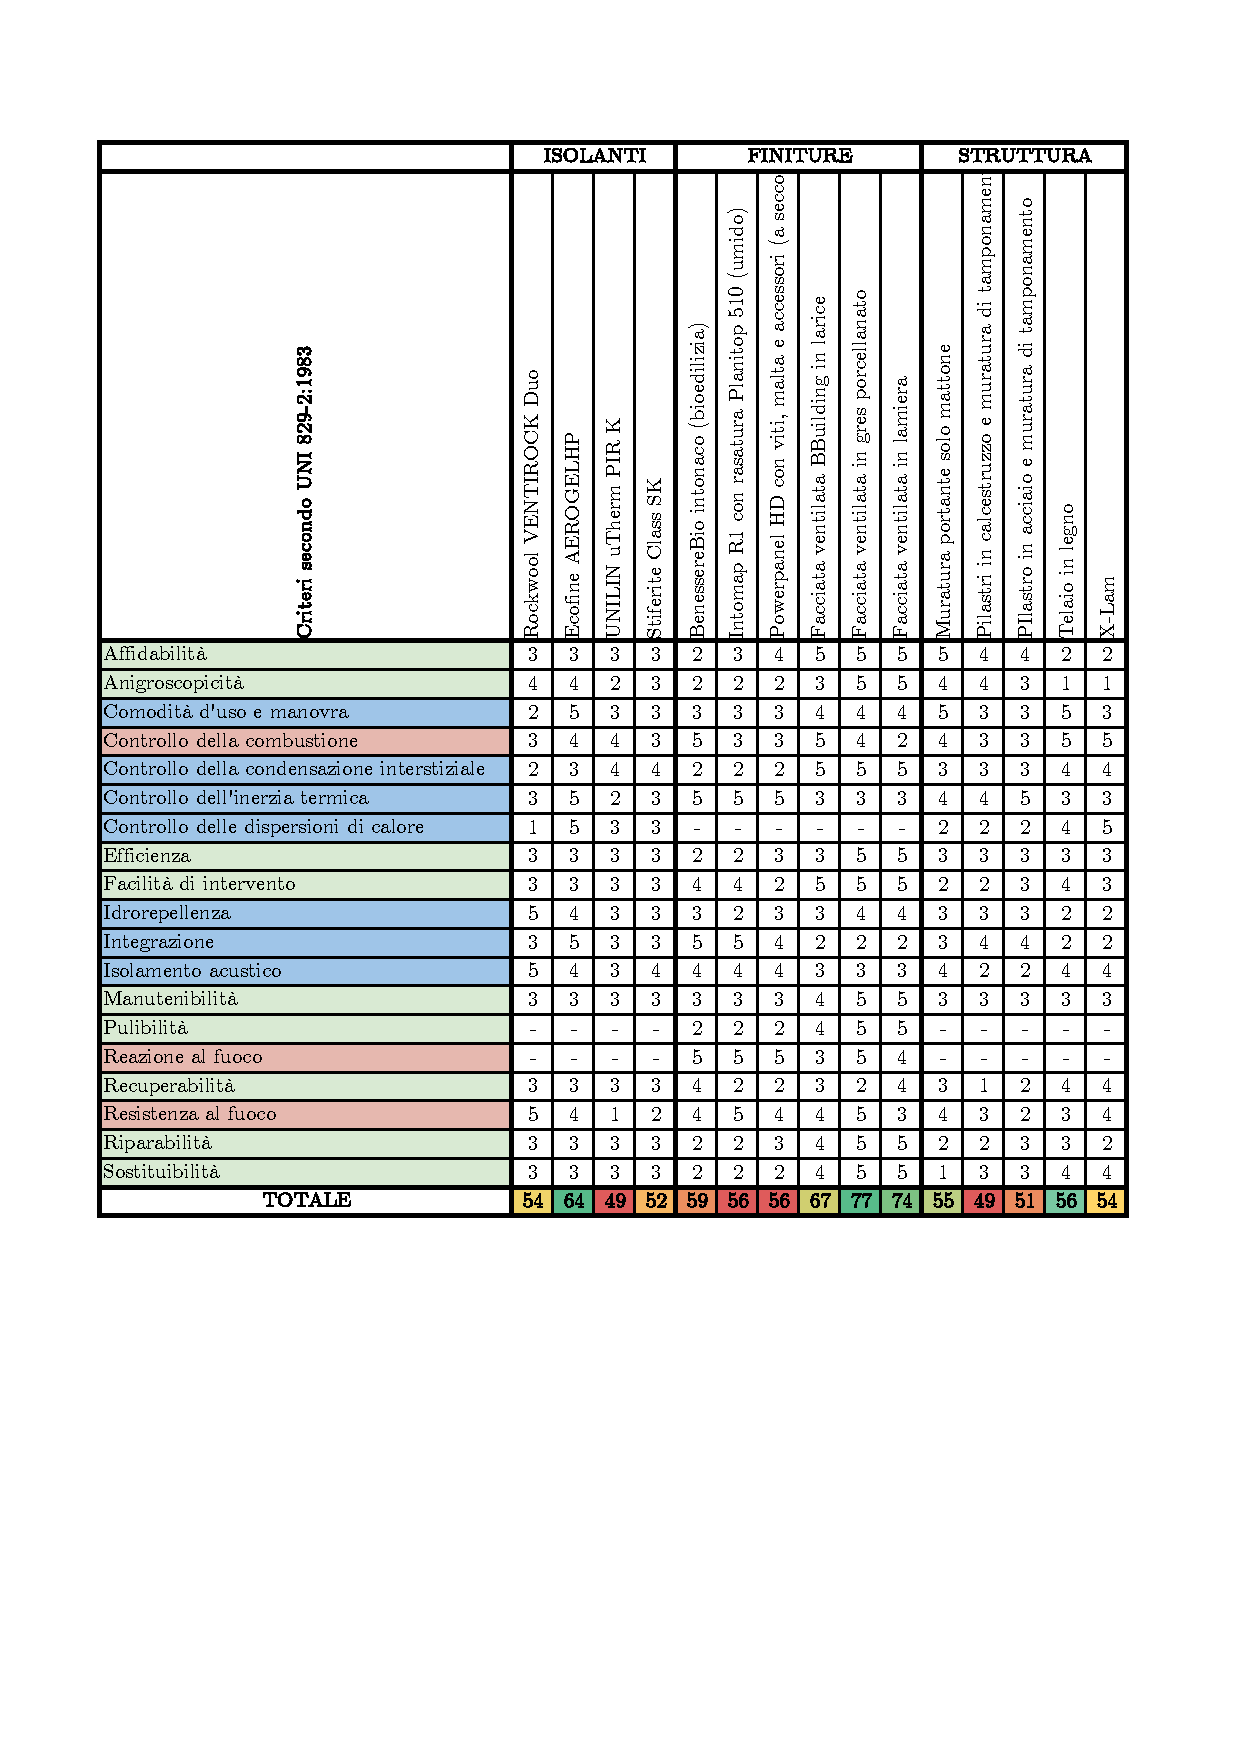
\includegraphics[width=0.9\textwidth]{img/AnalisiValore.pdf}
    \caption[Analisi del valore delle pareti esterne]{%
\scriptsize
Analisi del valore delle pareti esterni in cui è stato dato un punteggio da 1 a 5 per ogni campo considerato.
\textbf{Affidabilità:} Capacità di mantenere sensibilmente invariata nel tempo la propria qualità in condizioni d'uso determinate
\textbf{Anigroscopicità:} Attitudine a non subire mutamenti di aspetto e/o morfologia, di dimensione e comportamento in seguito ad assorbimento di acqua o di vapor d'acqua
\textbf{Comodità d'uso e manovra:} Attitudine a presentare opportune caratteristiche di funzionalità, di facilità d'uso, di manovrabilità
\textbf{Controllo della combustione:} Realizzazione e mantenimento di condizioni tali da produrre processi di combustione a massimo rendimento di trasformazione e minima produzione di scorie e sostanze inquinanti
\textbf{Controllo della condensazione interstiziale:} Attitudine ad evitare la formazione di acqua di condensa all'interno degli elementi
\textbf{Controllo dell'inerzia termica:} Attitudine ad attenuare entro opportuni valori l'ampiezza di oscillazione della temperatura e a ritardarne di una opportuna entità l'effetto
\textbf{Controllo delle dispersioni di calore:} Contenimento entro determinati livelli delle perdite di calore per conduzione, convezione e irraggiamento
\textbf{Efficienza:} Capacità costante di rendimento nel funzionamento
\textbf{Facilità di intervento:} Possibilità di operare ispezioni, manutenzione e ripristini in modo agevole
\textbf{Idrorepellenza:} Attitudine a non essere penetrato da fluidi liquidi
\textbf{Integrazione:} Attitudine alla connessione funzionale e dimensionale
\textbf{Isolamento acustico:} Attitudine a fornire un'adeguata resistenza al passaggio di rumori
\textbf{Manutenibilità:} Possibilità di conformità a condizioni prestabilite entro un dato periodo di tempo in cui è compiuta l'azione di manutenzione
\textbf{Pulibilità:} Attitudine a consentire la rimozione di sporcizia e sostanze indesiderate
\textbf{Reazione al fuoco:} Grado di partecipazione di un materiale combustibile ad un fuoco al quale è sottoposto
\textbf{Recuperabilità:} Attitudine alla riutilizzazione di materiali o di elementi tecnici dopo demolizione o rimozione
\textbf{Resistenza al fuoco:} Attitudine a conservare, entro limiti determinati, per un intervallo di tempo determinato, le prestazioni fornite
\textbf{Riparabilità:} Attitudine a ripristinare l'integrità, la funzionalità e l'efficienza di parti o oggetti guasti 
\textbf{Sostituibilità:} Attitudine a consentire la collocazione di elementi tecnici al posto di altri}
\label{fig:AnalisiValore}
\end{figure}